\begin{frame}
    \frametitle{Redes \textit{PON}}
    \begin{itemize}
        % \item Série de tecnologias de banda alargada que oferecem enormes
        % vantagens em cenários de fibra até à casa do cliente - arquiteturas de
        % ponto a ponto, capacidade para \textit{streams} triplas de alta
        % qualidade de voz...
        \item Tecnologias que oferecem vantagens em cenários de fibra até à casa do cliente.
        \item Em termos físicos uma rede \textit{PON} é constituída por:
        \textit{OLT - Optical Line Terminal}, \textit{ODN - Optical Distribution
        Network} e \textit{ONT - Optical Network Terminal}.
    \end{itemize}
\end{frame}

% \begin{frame}
%     \frametitle{Constituição das redes \textit{PON}}
%     \centering
%     \begin{figure}
%         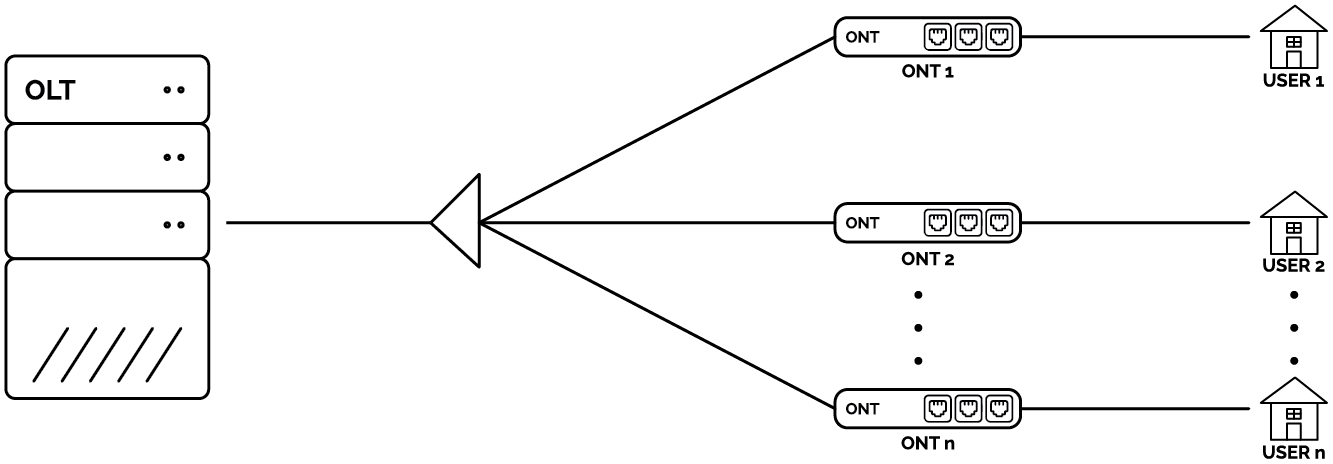
\includegraphics[width=0.9\textwidth]{./assets/estado_de_arte/rede_pon.png}
%     \end{figure}    
% \end{frame}    

\begin{frame}
    \frametitle{\textit{\textbf{AGORA}}}
    \begin{figure}
        
\includegraphics[width=0.6\textwidth]{./assets/estado_de_arte/alticelabs_logo.png}
    \end{figure}    
    \begin{itemize}
        \item O \textit{\textbf{AGORA}} é um \textit{Network Management System}.
        \item Assenta no modelo \textit{FCAPS}.
        \item \textit{FCAPS} - \textit{Fault, Configuration, Accountability,
        Performance and Security}.
        \item Escalável, programável, modular e simples.
    \end{itemize}    
\end{frame}    

\begin{frame}
    \frametitle{\textit{ZTP - Zero Touch Provision}}
    \begin{itemize}
        \item Módulo existente no \textit{\textbf{AGORA}} responsável pelo
        provisionamento automático dos equipamentos do tipo \textit{OLT}.
        \item O processo de aprovisionamento deste tipo de equipamentos é um
        processo bastante repetitivo e que, por isso, é um alvo preferencial de
        automatização.
    \end{itemize}    
\end{frame}    

\begin{frame}
    \frametitle{Ferramentas de automatização}
    \begin{itemize}
        \item \textit{CFEngine}
        \item \textit{Rudder}
        \item \textit{Ansible}
        \item \textit{Puppet}
        \item \textit{Juju}
    \end{itemize}    
\end{frame}    

\begin{frame}
    \frametitle{Comparação entre ferramentas de automatização}
    \begin{table}[H]
        \centering
        \begin{tabular}{lllll}
          \hline
                            & \textbf{Linguagem} & \textbf{Agente} & \textbf{SSH}  \\ \hline
          \textbf{CFEngine} & yaml               & yes              & yes          \\ \hline
          \textbf{Rudder}   & gui                & yes              & yes          \\ \hline
          \textbf{Ansible}  & yaml               & no               & yes          \\ \hline
          \textbf{Puppet}   & puppet             & yes              & yes          \\ \hline
          \textbf{Juju}     & yaml               & yes              & yes          \\ \hline
        \end{tabular}
        \caption{Comparação entre ferramentas de automatização}
        \label{tab:automation_tools_comparison}
      \end{table}
\end{frame}    

\begin{frame}
    \frametitle{\textit{Frameworks} para microsserviços}
    \begin{itemize}
        \item \textit{Spring Boot}
        \item \textit{Dropwizard}
        \item \textit{Go Micro}
        \item \textit{Moleculer}
    \end{itemize}    
\end{frame} 